\section{Besoins fonctionnels}
Lors de nos différents échanges avec le client nous avons pu identifier ses besoins pour ce projet. En effet, la réalisation de ce projet nécessite plusieurs parties:

\subsection{Partie Langue- Importance 5/}
Mettre en place une base de données qui utilise le niveau intensif du \textbf{LeFFF} pour former les différents mots du \textbf{lexique}.

\subsubsection{Génération des formes fléchies}
Ce besoin est le \textbf{besoin principal} de notre projet. Si notre base de données doit contenir en plus des mots du lexique toutes les expressions possibles qui vont avec, le projet aurait été vraiment très simple (c'est à dire un site internet qui permet d'enregistrer et de manipuler des informations). En effet, une \textbf{génération dynamique} des formes fléchies permettra une \textbf{réduction} considérable de la \textbf{taille du lexique} à enregistrer dans la base de données. Pour remédier à ce problème, il nous faut donc mettre en place un outil qui respecte les \textbf{règles linguistique} pour générer les formes fléchies.

\subsubsection{Base de Données - Importance 5/5}


{Nous allons utiliser une \textbf{base de données relationnelle}. A première vue il aurait été plus judicieux d'utiliser une base de données non relationnelle du fait du nombre volumineux de données à traiter. Néanmoins le choix d'utiliser ici une base de données relationnelle nous permettra une plus \textbf{simple} gestion des données en particulier pour la recherche. Afin \textbf{d'optimiser} la \textbf{recherche} nous utiliserons une ou plusieurs de ces 3 solutions : 
\begin{itemize}
\item Des \textbf{fichiers triés}, rapide pour la recherche (recherche dichotomique), mais lents pour l'insertion et la suppression.
\item Des \textbf{fichiers hachés} efficaces pour les sélections avec égalité.
\item Des \textbf{index} (pour chaque lettre de l'alphabet) pour permettre d'améliorer certaines opérations sur un fichier.
\end{itemize}\par}

\subsubsection{Rechercher un lexique - Importance 5/5}

{Nous offrirons la possibilité de rechercher un \textbf{lexique} de la même manière qu'un dictionnaire, mais aussi en permettant de le chercher en fonction de son \textbf{lemme} et \textbf{lexème} (sa définition ou synonyme). Par exemple l'entrée en recherche "content", nous pourrons retrouver en sortie "content", "heureux", "être à la fête", "être aux anges", "être gai comme un pinson",... Par la suite, nous pourrons afficher toutes les formes possibles pour chacun des résultats retournés comme par exemple singulier, pluriel, ou temps conjugués pour les verbes. Un exemple de test réalisable serait de rechercher un mot et de refaire une recherche avec l'un des résultats obtenus pour comparer les deux recherches.\par}

\begin{figure}[ht]
    \centering
    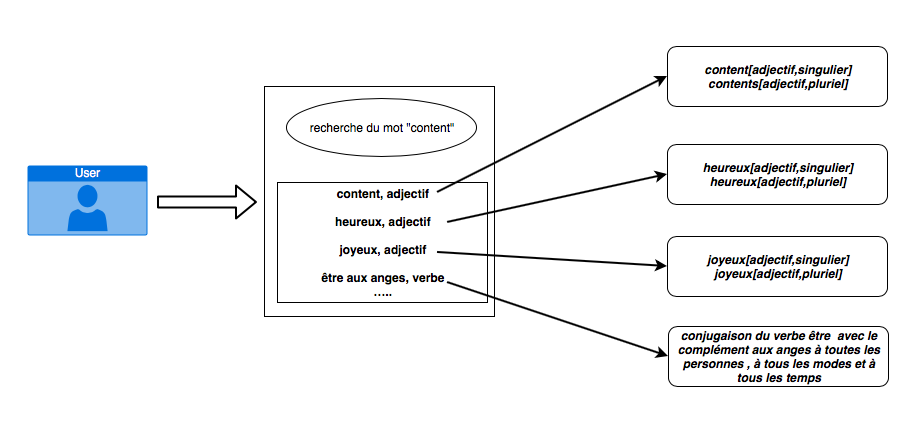
\includegraphics[scale=0.5]{exemple.png}
    \caption{Scénario d'utilisation pour la recherche d'un mot }
\end{figure}
\newpage

\subsubsection{Transducteur - Importance 5/5}


La composition des \textbf{transducteurs} nous permettra de construire un \textbf{lexique} spécifique à la nature de l'entrée, nous pouvons réaliser des \textbf{transducteurs} par exemple qui vont \textbf{conjuguer} des verbes, d'autres qui vont \textbf{transformer} du masculin ou féminin, du singulier ou pluriel, ou \textbf{inversement}. Les algorithmes de construction des transducteurs pourront prendre en compte des \textbf{filtres} afin d'affiner la recherche et la rendre plus rapide.Chaque \textbf{arcs} correspondra à une \textbf{spécification} du mot (symboles signifiant la nature et la morphologie d'un mot).



{Il faudra mettre en place un transducteur qui aura pour fonction de récupérer le radical d'un mot fourni pour se faire nous utiliserons plusieurs automates finis afin de détecter sa catégorie grammaticale, pour ensuite connaître sa forme dans le but de retourner son radical.\par}

{Inversement, à partir d'un autre transducteur, celui ci devra retourner toutes ses formes.\par}

\begin{figure}[ht]
    \centering
    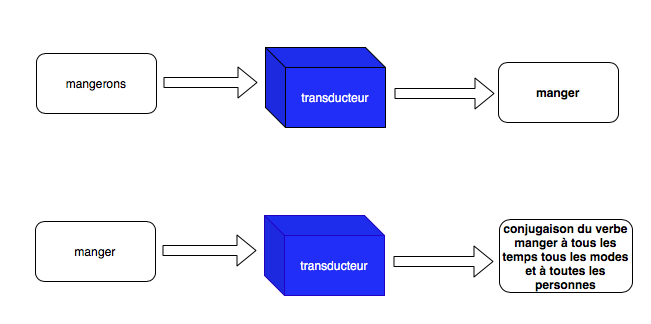
\includegraphics[scale=0.5]{transducteur.png}
    \caption{transducteur }
\end{figure}

\newpage

\subsubsection{Unificateur - Importance 5/5}{
\textbf{L'unificateur} est l'algorithme qui va nous permettre de \textbf{lier} plusieurs \textbf{mots} afin d'en tirer le \textbf{sens}, pour ce faire, il faut faire \textbf{l'union des informations} sur ces mots. S'il y a une \textbf{contradiction} avec ces informations, alors la phrase est \textbf{mal formée} et dans ce cas aucun sens ne sera retourné, sinon on pourra voir quel est le sens de l'expression formée.\par}

\begin{figure}[ht]
    \centering
    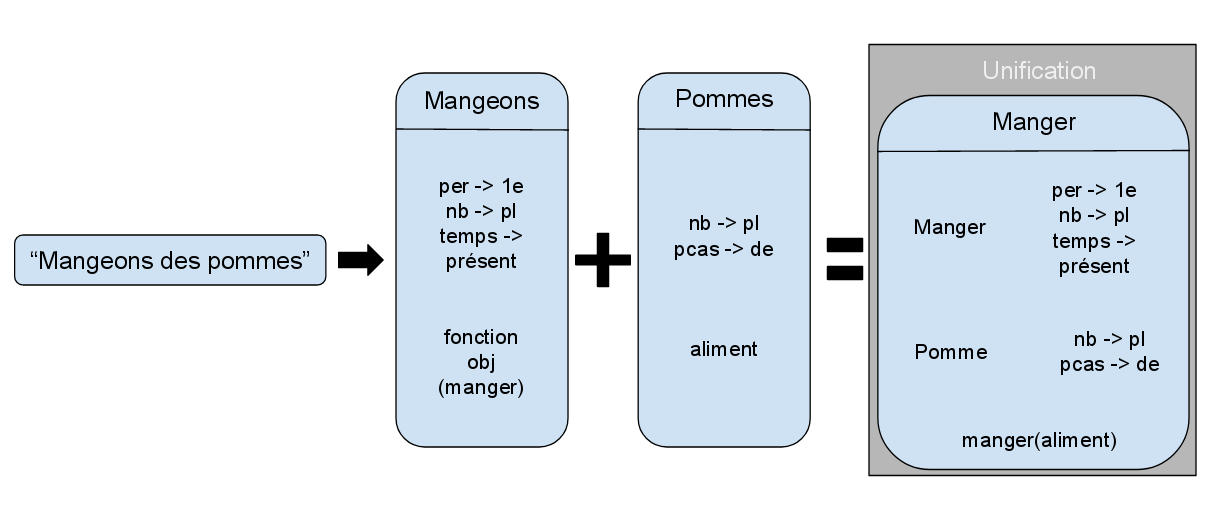
\includegraphics[scale=0.4]{unificateur.png}
    \caption{Unificateur }
\end{figure}

{Les mots utilisés sur \textbf{l'unificateur} utiliserons une \textbf{sous-structure commune} afin de faciliter et de rendre sensée cette opération, puis à l'aide de la \textbf{théorie de substitution des ensembles}, nous pourrons \textbf{optimiser} la construction de nos formules. Celles-ci nous permettrons par la suite d'\textbf{améliorer} la \textbf{rapidité} de l'algorithme de recherche, ainsi que la \textbf{mémoire} utilisée.\par}

